\documentclass{article}
\usepackage[spanish]{babel}
\usepackage[numbers,sort&compress]{natbib}
\usepackage{graphicx}

\title{Simulaci\'{o}n del movimiento Browniano y examinaci\'{o}n de los efectos de las dimenciones en los tiempos de regreso al origen de una part\'{i}cula}
\author{Isaac Estrada Garc\'{i}a }

\begin{document}

\maketitle

\section{Introducci\'{o}n}
El movimiento Browniano es un modelo matem\'{a}tico de una part\'{i}cula que describe la "danza'' aleatoria de las part\'{i}culas que se debe\citep{mov} a la agitaci\'{o}n molecular en la que se hayan inmersas.

En este trabajo los objetivos principales son modelar sistem\'{a}ticamente el movimiento Browniano de una part\'{i}cula de una a ocho dimensiones del espacio, as\'{i} como tambi\'{e}n examinar el tiempo de regreso al origen de la part\'{i}cula analizando su caminata pseudoaleatoria.

\section{Hip\'{o}tesis}
Es posible que la probabilidad sea nula conforme las dimensiones vayan aumentando y de la misma manera los regresos al origen.

\section{Objetivos}
Simular el movimiento Browniano\citep{elis} de una part\'{i}cula examinando los efectos de la dimensi\'{o}n en el tiempo de regreso al origen para dimensiones de 1 a 8 en incrementos lineales de uno, variando el n\'{u}mero de pasos de la caminata como potencias de dos, con exponentes de 5 a 10 en incrementos lineales de uno, con 50 repeticiones del experimento para cada combinaci\'{o}n y graficar los resultados en una sola figura con diagramas de caja-bigote. 

\section{Simulaci\'{o}n y Resultados}

La simulaci\'{o}n del movimiento Browniano se realiza con lenguaje de programaci\'{o}n Python. La codificaci\'{o}n se encuentra en el repositorio de "simulacion" da como resultado una grafica caja-bijote que describe los pasos que toma la part\'{i}cula al llegar al origen partiendo de el, se realizan 50 experimentos para 6 distintas caminatas y en 8 dimenciones, posterior se calcula el tiempo medido en pasos de regreso al origen.

En la figura \ref{fig} se muestran los resultados obtenidos por la simulaci\'{o}n, donde se puede observar una tendencia decreciente de regresos al origen conforme aumentan las dimenciones.


\begin{figure}
  \centering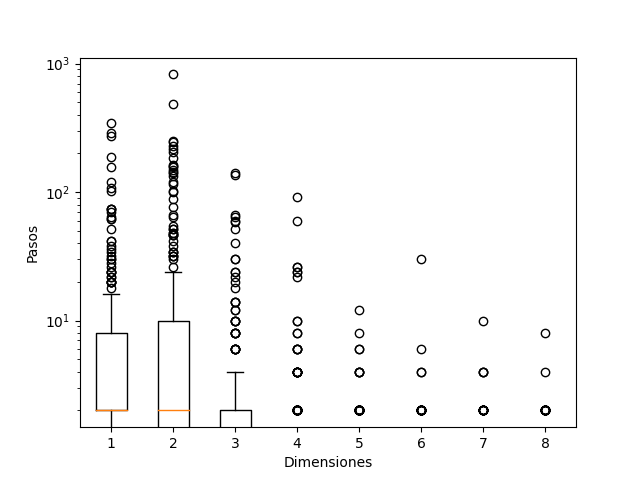
\includegraphics[width=0.9\textwidth]{p1_2.png}
  \caption{Regresos al origen de una part\'{i}cula simulado sistematicamente por el modelo movimiento Browniano.}
  \label{fig}
\end{figure} 



\section{Conclusi\'{o}n}

Mientras m\'{a}s dimenciones existan en el movimiento  pseudoaliatorio de una part\'{i}cula, menor son las veces que pasa por su origen.

\bibliography{p1}
\bibliographystyle{plainnat}
 
\end{document}
